\documentclass[11pt, a4paper, tikz]{article}

\usepackage[english]{babel} %language
\usepackage[utf8]{inputenc} %UTF-8 encoding
\usepackage[margin=0.5in]{geometry} %smaller margin
\usepackage{amssymb} %\nexists \mathbb
\usepackage{amsmath}
\usepackage{amsthm}
\usepackage{graphicx}
\usepackage{polynom}
\usepackage{mathtools}

\usepackage{xlop}
\usepackage[dvipsnames]{xcolor}
\usepackage{tcolorbox}

\definecolor{formulationFrameColor}{RGB}{150,160,190}
\definecolor{formulationBackgroundColor}{RGB}{240,245,250}

\newtcolorbox{formulationBox}{
	colframe=formulationFrameColor,
	colback=formulationBackgroundColor
}

\usepackage{tikz}   
\usepackage{pgfplots}

\pgfplotsset{compat=1.6}

\pgfplotsset{soldot/.style={color=red,only marks,mark=*}} \pgfplotsset{holdot/.style={color=red,fill=white,only marks,mark=*}}

\pgfplotsset{compat=newest} % used to declare my style command.  

\newcommand{\newpara}{
	\vskip 2mm
}

\newcommand{\centsection}[1]{
	\section*{\centering{#1}}
}

\newcommand{\centsubsection}[1]{
	\subsection*{\centering{#1}}
}

\newcommand{\myOver}[2]{
	\ensuremath{\overset{\kern2pt #1}{#2}}
}

\newcommand{\final}[1]{
	$\mathcal{F}($#1$)$
}

\newcommand{\Lim}[1]{\raisebox{0.5ex}{\scalebox{0.8}{$\displaystyle \lim_{#1}\;$}}}
\newcommand{\Sum}[2]{\displaystyle \sum_{#1}^{#2}}

\begin{document}
	\title{\textbf{Chapter 1 — Part A}}
	\author{Ander Aguinaga San Sebastián}
	\date{23/09/2023}
	\maketitle
	%\setcounter{section}{3}
	\centsection{Exercise 1}
	
	\begin{formulationBox}
		Suppose $f:[a,b]\rightarrow\mathbb{R}$ is a bounded function such that \[L(f,P,[a,b]) = U(f,P,[a,b])\] for some partition $P$ of $[a,b]$. Prove that $f$ is a constant function on $[a,b]$.
	\end{formulationBox}
	
	By definition,
	\begin{equation*}
		L(f, P, [a, b]) = \sum_{j=1}^{n}(x_j-x_{j-1})\inf_{[x_{j-1,x_j}]}f
	\end{equation*}
	and
		\begin{equation*}
		U(f, P, [a, b]) = \sum_{j=1}^{n}(x_j-x_{j-1})\sup_{[x_{j-1,x_j}]}f
	\end{equation*}
	.
	\newpara
	Therefore, for the lower and upper Riemann sums to be equal, the infimum and the supremum of $f$ in each of the $[x_{j-1},x_j]$ subintervals need to be the same. To prove this only happens when $f$ in constant, let's suppose there exist $x_1, x_2\in\mathbb{R}$ such that $f(x_1) < f(x_2)$ in an interval $[\alpha,\beta]$. By definition,
	\begin{equation*}
		\inf_{[\alpha,\beta]}f \leq f(x_1) < f(x_2) \leq  \sup_{[\alpha,\beta]}f \implies \inf_{[\alpha,\beta]}f < \sup_{[\alpha,\beta]}f
	\end{equation*}. Therefore, we need the function to be constant in order for the infimum and the supremum to be equal to each other.
	$\qed$
	
	\centsection{Exercise 2}
	
	\begin{formulationBox}
		Suppose $a\geq s<t\geq b$. Define $f:[a,b]\rightarrow\mathbb{R}$ by
		\[
			f(x) =
			\begin{cases}
				1 &\quad s<x<t\\
				0 &\quad \textrm{otherwise.}\\ 
			\end{cases}
		\]
		Prove that $f$ is Riemann integrable on $[a,b]$ and that $\int_a^bf=t-s$.
	\end{formulationBox}
	
	\begin{center}
	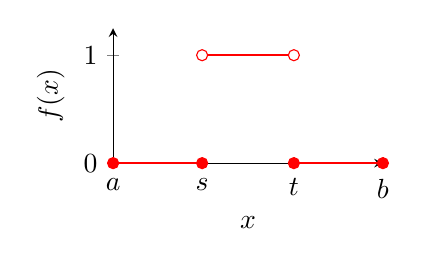
\begin{tikzpicture}
		\begin{axis}[
			axis lines = left,
			xmin=0,xmax=1,
			xlabel = $x$,
			ylabel = {$f(x)$},
			xtick={0, 0.33,0.67, 1},
			xticklabels={$a$, $s$, $t$, $b$},
			ytick={0, 0.4},
			yticklabels={$0$,$1$},
			unbounded coords=jump,ymax=0.5,
			scale=0.5,
			axis equal image
			]
			
			\addplot[thick, domain=0:0.33,red] {0};
			\addplot[thick, domain=0.33:0.67,red] {0.4};
			\addplot[thick, domain=0.67:1,red] {0};
			%\draw[dotted] (axis cs:0.33,0) -- (axis cs:0.33,1);
			%\draw[dotted] (axis cs:0.67,0) -- (axis cs:0.67,1);
			\addplot[holdot] coordinates{(0.33,0.4)(0.67,0.4)};
			\addplot[soldot] coordinates{(0,0)(0.33,0)(0.67,0)(1,0)};
		\end{axis}
	\end{tikzpicture}
	\end{center}
	\newpara
	Let's first calculate the upper Riemann integral:
	\begin{align*}
		U(f, [a,b]) \leq \inf_PU(f, P, [a,b]) = \inf_P\sum_{j=1}^n(x_j-x_{j-1})\sup_{[x_{j-1},x_j]}f\\
		=\inf_P\sum_{j=1}^\alpha(x_j-x_{j-1})\sup_{[x_{j-1},x_j]}f+\inf_P\sum_{j=\alpha+1}^\beta(x_j-x_{j-1})\sup_{[x_{j-1},x_j]}f+\inf_P\sum_{j=\beta+1}^n(x_j-x_{j-1})\sup_{[x_{j-1},x_j]}f\\
		=0+\inf_P\sum_{j=\alpha+1}^\beta(x_j-x_{j-1})\cdot1+0=\inf_P(x_\beta-x_{\alpha})=t-s
	\end{align*}
	Where $\alpha,\beta\in\mathbb{R}$ such that $x_\alpha=s$ and $x_\beta=t$, and $n$ is the number of points in the partition.
	
	Likewise:
	\begin{align*}
		L(f, [a,b]) \geq \sup_PL(f, P, [a,b]) = \sup_P\sum_{j=1}^n(x_j-x_{j-1})\inf_{[x_{j-1},x_j]}f\\	=\sup_P\sum_{j=1}^\alpha(x_j-x_{j-1})\inf_{[x_{j-1},x_j]}f+\sup_P\sum_{j=\alpha+1}^\beta(x_j-x_{j-1})\inf_{[x_{j-1},x_j]}f+\sup_P\sum_{j=\beta+1}^n(x_j-x_{j-1})\inf_{[x_{j-1},x_j]}f\\
		=0+\sup_P\sum_{j=\alpha+1}^\beta(x_j-x_{j-1})\cdot1+0=\sup_P(x_\beta-x_\alpha)=t-s
	\end{align*}
	I'm getting confused with the notation and I don't think it's that important to enter in details right now (?).
	
	\centsection{Exercise 3}
	
	\begin{formulationBox}
		Suppose $f:[a,b]\rightarrow\mathbb{R}$ is a bounded function. Prove that $f$ is Riemann integrable if and only if for each $\epsilon>0$, there exists a partition $P$ of $[a,b]$ such that \[U(f,P,[a,b]) - L(f,P,[a,b]) < \epsilon.\]
	\end{formulationBox}
	
	To prove the first implication, we define $I$ to be the value of $\int_{a}^{b}f$. As $f$ is Riemann integrable, we have \begin{align*}
		U(f,[a,b])=L(f,[a,b])=I\\
		\implies\inf_PU(f,P,[a,b])=\sup_PL(f,P,[a,b])=I\\ \implies\inf_PU(f,P,[a,b])-\sup_PL(f,P,[a,b])=0
	\end{align*}.
	By definition of infimum, there exists a partition $P$ such that $U(f,P,[a,b])< I+\epsilon$ for every $\epsilon>0$. Similarly, there exists a partition $P$ such that $L(f,P,[a,b])>I-\epsilon$ for every $\epsilon>0$.
	
	For example, if we choose $\epsilon_0>0$ as the desired upper bound, there exists a partition $P$ so that
	\begin{align*}
		U(P,f,[a,b])-L(P,f,[a,b])<(I+\frac{\epsilon_0}{3})-(I-\frac{\epsilon_0}{3})=\frac{2}{3}\epsilon_0 < \epsilon_0
	\end{align*}.
	
	We now prove the second implication. Minding that \[U(f,[a,b])=\inf_PU(f,P,[a,b])\leq U(f,P,[a,b])\] and \[L(f,[a,b])=\sup_PL(f,P,[a,b])\geq L(f,P,[a,b])\], we get \[U(f,[a,b])-L(f,[a,b])<\epsilon\]. If $f$ weren't Riemann integrable, then \[U(f,[a,b])-L(f,[a,b])=\Delta\], so there would exist an $\epsilon_0>0$ such that $\epsilon<\Delta$, contradicting the initial hypothesis. Therefore, $f$ needs to be Riemann integrable.
	$\qed$
\end{document}